\documentclass{article}
\usepackage{fullpage}
\usepackage[MeX]{polski}
\usepackage[utf8]{inputenc}
\usepackage{amsfonts}
\usepackage{amssymb}
\usepackage{graphicx}

\author{Piotr Dobrowolski, 291528}
\title{Serwis cytatów - sentencji \\ Opis protokołu}
\date{\today}
\frenchspacing

\begin{document}
\maketitle
\tableofcontents
\clearpage

\section{Streszczenie}
Niniejszy dokument opisuje specyfikację protokołu serwisu cytatów-sentencji.
Składa się z następujących sekcji:
\begin{itemize}
\item opis celów protokołu,
\item opis założeń,
\item opis formatu komunikatów,
\item opis stanów.
\end{itemize}


\section{Opis celów protokołu}
Protokół ma obsługiwać sposób szybkiego przekazywania krótkiego tekstu (cytatu/sentencji).
Cytaty będą udostępniane klientom przez serwer.
Protokołu jest nastawiony na szybkość kosztem niezawodności dostarczanych tekstów.


\section{Terminologia}
\begin{description}
\item[Klient: ] użytkownik instancji protokołu, który chce pobrać cytat,
\item[Serwer: ] użytkownik udostępniający teksty klientom,
\item[Cytat: ] będę używał wymiennie z tekst, sentencja. Są to dane tekstowe przesyłane protokołem,
\item[Długi cytat: ] jest to cytat, który nie mieści się w jednym komunikacie, i należy go podzielić.
%może dodać - klient oczekujący, klient rozpoznany, coś takiego?
\end{description}


\section{Założenia}
\subsection{Połączenie}
Serwer odpowiada na żądania klientów. W jednej chwili może obsługiwać wielu na raz.
\subsection{Wykorzystanie innych protokołów}
Protokół działa w warstwie aplikacji. 
Zależy nam na szybkości, a komunikacja nie musi być niezawodna,
także do transportu będzie użyty protokół UDP.
\subsection{Model komunikacji}
Protokół działa w modelu klient-serwer. Pojedynczy serwer z cytatami, udostępnia je wielu klientom.
Jak przedstawiono na diagramie poniżej.
\begin{center}
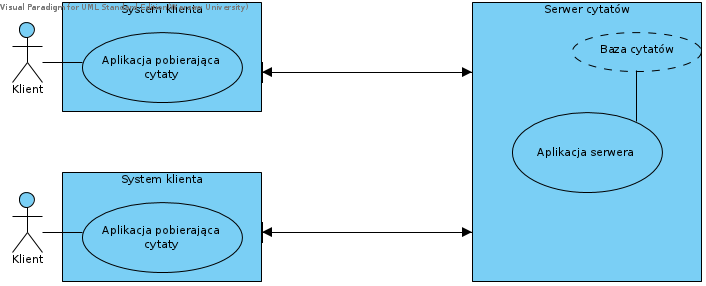
\includegraphics[scale=0.6]{model.png}
\end{center}

\section{Opis formatu komunikatów}
\subsection{Założenia}
\begin{itemize}
\item Protokół stosuje sieciowy porządek oktetów w liczbach,
\item Dopuszczalne uzupełnianie formatu zerami. 
%\item coś jeszcze
\end{itemize}
\subsection{Typy pomocnicze}
\begin{verbatim}
PART_ID_T {
   uint8    part_nr     = 0;
   uint8    all_parts   = 1;
}
\end{verbatim}
Typ ten służy do odróżnienia paczki z tekstem, tak aby później można było poskładać długi cytat w dobrej kolejności.\\
Części \verb+part_nr+ numerowane są od $0$.

\begin{verbatim}
QUOT_T {
   PART_ID_T            part_id;
   uint16               quot_length = max_quot_length;
   octet[quot_length]   quot;
}
\end{verbatim}
\verb+quot_length+ - pole zawierające długość cytatu w oktetach.\\
Struktura zachowuje cytat (jedną z części cytatu długiego). Oraz identyfikator jednoznacznie określający która jest to część.

\subsection{Typy komunikatów}
\begin{verbatim}
QUOT_REQUEST_MSG_T {
   /*empty messsage*/
}
\end{verbatim}
Zgłoszenie się klienta.
Służy do wysłania do serwera prośby o cytat. Jest to pusta struktura.

\begin{verbatim}
QUOT_RESPONSE_MSG_T {
   uint16      id;
   QUOT_T      quotation;
}
\end{verbatim}
Struktura komunikatu wysyłanego z serwera do klienta, \verb+id+ oznacza identyfikator wysłanego
cytatu (aby nie dopuścić do wymieszania komunikatów).

\section{Opis wymienianych komunikatów}
Protokół posługuje się dwoma komunikatami: \verb+QUOT_REQUEST_MSG+ i \verb+QUOT_RESPONSE_MSG+. 
(W nawiasach podane są argumenty, a po dwukropku typ komunikatu).
\subsection{Wysyłane przez klienta}
\subsubsection{Zgłaszanie się do serwera}
\verb+QUOT_REQUEST_MSG():     QUOT_REQUEST_MSG_T+\\
Klient posługuje się pustym komunikat aby zgłosić chęć pobrania cytatu z serwera.
Po odebraniu tego komunikatu serwer przygotowuje (losuje, dzieli) cytat i przechodzi do stanu wysyłania cytatu do tego klienta.
\subsection{Wysyłane przez serwer}
\subsubsection{Komunikat z danymi}
\verb+QUOT_RESPONSE_MSG(id, quotation):     QUOT_RESPONSE_MSG_T+\\
W komunikacie zawarty jest:
\begin{itemize}
\item \verb+id:+ identyfikator cytatu, potrzebny w celu jednoznacznej identyfikacji cytatu.
\item \verb+quotation:+ dane, tekst zawierający cytat, \verb+quotataion.quot:+ zawiera tekst cytatu.
Znaki kodowane są za pomocą systemu UTF-8.
\end{itemize}
\section{Opis stanów}

\subsection{Klient}
Klient wysyła żądanie do serwera (\verb+QUOT_REQUEST_MSG()+), w chwili oczekiwania jest w
stanie \verb+WAIT_FOR_QUOT+ a następnie zbiera pakiety odebrane z serwera.
Klient identyfikuje cytat po odebraniu pierwszej części (zapisuje id). I na podstawie id będzie dalej pobierał brakujące
części.
Podczas wysłania żądania zostaje zainicjowane odliczanie czasu, jeżeli czas oczekiwania na części cytatu które nie doszły przekroczy 
\verb+timeout+ to pobieranie cytatu zostaje anulowane. \verb+timeout+ ustalane jest przez autora implementacji.
\subsection{Serwer}
Serwer odbiera od klientów żądania \verb+QUOT_REQUEST_MSG()+ Przydziela temu zapytaniu identyfikator.
Następnie dzieli cytat (jeżeli jest długi) zgodnie z \verb+max_quot_length+
i za pomocą komunikatów \\ \verb+QUOT_RESPONSE_MSG(id, quotation)+ wysyła wiadomość do danego klienta.

\section{Numery}
\begin{itemize}
\item \verb+max_quot_length = 1024+ ustalany w czasie kompilacji
\item \verb+timeout = 3+ proponowany
\end{itemize}

\end{document}
